%% abtex2-modelo-relatorio-tecnico.tex, v<VERSION> laurocesar
%% Copyright 2012-<COPYRIGHT_YEAR> by abnTeX2 group at http://www.abntex.net.br/ 
%%
%% This work may be distributed and/or modified under the
%% conditions of the LaTeX Project Public License, either version 1.3
%% of this license or (at your option) any later version.
%% The latest version of this license is in
%%   http://www.latex-project.org/lppl.txt
%% and version 1.3 or later is part of all distributions of LaTeX
%% version 2005/12/01 or later.
%%
%% This work has the LPPL maintenance status `maintained'.
%% 
%% The Current Maintainer of this work is the abnTeX2 team, led
%% by Lauro César Araujo. Further information are available on 
%% http://www.abntex.net.br/
%%
%% This work consists of the files abntex2-modelo-relatorio-tecnico.tex,
%% abntex2-modelo-include-comandos and abntex2-modelo-references.bib
%%

% ------------------------------------------------------------------------
% ------------------------------------------------------------------------
% abnTeX2: Modelo de Relatório Técnico/Acadêmico em conformidade com 
% ABNT NBR 10719:2015 Informação e documentação - Relatório técnico e/ou
% científico - Apresentação
% ------------------------------------------------------------------------ 
% ------------------------------------------------------------------------

\documentclass[
	% -- opções da classe memoir --
	12pt,				% tamanho da fonte
	openany,			% capítulos começam em pág ímpar (insere página vazia caso preciso)
	twoside,			% para impressão em recto e verso. Oposto a oneside
	a4paper,			% tamanho do papel. 
	% -- opções da classe abntex2 --
	%chapter=TITLE,		% títulos de capítulos convertidos em letras maiúsculas
	%section=TITLE,		% títulos de seções convertidos em letras maiúsculas
	%subsection=TITLE,	% títulos de subseções convertidos em letras maiúsculas
	%subsubsection=TITLE,% títulos de subsubseções convertidos em letras maiúsculas
	% -- opções do pacote babel --
	english,			% idioma adicional para hifenização
	french,				% idioma adicional para hifenização
	spanish,			% idioma adicional para hifenização
	brazil,				% o último idioma é o principal do documento
	]{abntex2}


% ---
% PACOTES
% ---

% ---
% Pacotes fundamentais 
% ---
\usepackage{lmodern}			% Usa a fonte Latin Modern
\usepackage[T1]{fontenc}		% Selecao de codigos de fonte.
\usepackage[utf8]{inputenc}		% Codificacao do documento (conversão automática dos acentos)
\usepackage{indentfirst}		% Indenta o primeiro parágrafo de cada seção.
\usepackage{color}				% Controle das cores
\usepackage{graphicx}			% Inclusão de gráficos
\usepackage{microtype} 			% para melhorias de justificação
% ---

% ---
% Pacotes adicionais, usados no anexo do modelo de folha de identificação
% ---
\usepackage{multicol}
\usepackage{multirow}
% ---
	
% ---
% Pacotes adicionais, usados apenas no âmbito do Modelo Canônico do abnteX2
% ---
\usepackage{lipsum}				% para geração de dummy text
% ---

% ---
% Pacotes de citações
% ---
\usepackage[brazilian,hyperpageref]{backref}	 % Paginas com as citações na bibl
\usepackage[alf]{abntex2cite}	% Citações padrão ABNT

% ---
% Pacotes pessoais
% ---
\usepackage{listings}				% para inclusão de códigos-fonte no documento
% ---

% --- 
% CONFIGURAÇÕES DE PACOTES
% --- 

% ---
% Configurações do pacote backref
% Usado sem a opção hyperpageref de backref
\renewcommand{\backrefpagesname}{Citado na(s) página(s):~}
% Texto padrão antes do número das páginas
\renewcommand{\backref}{}
% Define os textos da citação
\renewcommand*{\backrefalt}[4]{
	\ifcase #1 %
		Nenhuma citação no texto.%
	\or
		Citado na página #2.%
	\else
		Citado #1 vezes nas páginas #2.%
	\fi}%
% ---

% ---
% Informações de dados para CAPA e FOLHA DE ROSTO
% ---
\titulo{Central de controle em domótica via Internet}
\autor{Gabriel Marques de Melo}
\local{Brasil}
\data{2018}
\instituicao{%
  Universidade Federal de Lavras
  \par
  Departamento de Engenharia
  \par
  Graduação em Ciência da Computação}

\tipotrabalho{Relatório técnico}
% O preambulo deve conter o tipo do trabalho, o objetivo, 
% o nome da instituição e a área de concentração 
\preambulo{Relatório técnico com o objetivo de documentação e apresentação do projeto desenvolvido na Universidade Federal de Lavras, no curso de Ciência da Computação.}
% ---

% ---
% Configurações de aparência do PDF final

% alterando o aspecto da cor azul
\definecolor{blue}{RGB}{41,5,195}

% informações do PDF
\makeatletter
\hypersetup{
     	%pagebackref=true,
		pdftitle={\@title}, 
		pdfauthor={\@author},
    	pdfsubject={\imprimirpreambulo},
	    pdfcreator={LaTeX with abnTeX2},
		pdfkeywords={abnt}{latex}{abntex}{abntex2}{relatório técnico}, 
		colorlinks=true,       		% false: boxed links; true: colored links
    	linkcolor=blue,          	% color of internal links
    	citecolor=blue,        		% color of links to bibliography
    	filecolor=magenta,      		% color of file links
		urlcolor=blue,
		bookmarksdepth=4
}
\makeatother
% --- 

% --- 
% Espaçamentos entre linhas e parágrafos 
% --- 

% O tamanho do parágrafo é dado por:
\setlength{\parindent}{1.3cm}

% Controle do espaçamento entre um parágrafo e outro:
\setlength{\parskip}{0.2cm}  % tente também \onelineskip

% ---
% compila o indice
% ---
\makeindex
% ---

% ----
% Início do documento
% ----
\begin{document}

% Seleciona o idioma do documento (conforme pacotes do babel)
%\selectlanguage{english}
\selectlanguage{brazil}

% Retira espaço extra obsoleto entre as frases.
\frenchspacing 

% ----------------------------------------------------------
% ELEMENTOS PRÉ-TEXTUAIS
% ----------------------------------------------------------
% \pretextual

% ---
% Capa
% ---
\imprimircapa
% ---

% ---
% Folha de rosto
% (o * indica que haverá a ficha bibliográfica)
% ---
\imprimirfolhaderosto*
% ---

\iffalse
% ---
% Anverso da folha de rosto:
% ---

{
\ABNTEXchapterfont

\vspace*{\fill}

Conforme a ABNT NBR 10719:2015, seção 4.2.1.1.1, o anverso da folha de rosto
deve conter:

\begin{alineas}
  \item nome do órgão ou entidade responsável que solicitou ou gerou o
   relatório; 
  \item título do projeto, programa ou plano que o relatório está relacionado;
  \item título do relatório;
  \item subtítulo, se houver, deve ser precedido de dois pontos, evidenciando a
   sua subordinação ao título. O relatório em vários volumes deve ter um título
   geral. Além deste, cada volume pode ter um título específico; 
  \item número do volume, se houver mais de um, deve constar em cada folha de
   rosto a especificação do respectivo volume, em algarismo arábico; 
  \item código de identificação, se houver, recomenda-se que seja formado
   pela sigla da instituição, indicação da categoria do relatório, data,
   indicação do assunto e número sequencial do relatório na série; 
  \item classificação de segurança. Todos os órgãos, privados ou públicos, que
   desenvolvam pesquisa de interesse nacional de conteúdo sigiloso, devem
    informar a classificação adequada, conforme a legislação em vigor; 
  \item nome do autor ou autor-entidade. O título e a qualificação ou a função
   do autor podem ser incluídos, pois servem para indicar sua autoridade no
   assunto. Caso a instituição que solicitou o relatório seja a mesma que o
   gerou, suprime-se o nome da instituição no campo de autoria; 
  \item local (cidade) da instituição responsável e/ou solicitante; NOTA: No
   caso de cidades homônimas, recomenda-se o acréscimo da sigla da unidade da
   federação.
  \item ano de publicação, de acordo com o calendário universal (gregoriano),
  deve ser apresentado em algarismos arábicos.
\end{alineas}

\vspace*{\fill}
}

% ---
% Agradecimentos
% ---
\begin{agradecimentos}
O agradecimento principal é direcionado a Youssef Cherem, autor do
\nameref{formulado-identificacao} (\autopageref{formulado-identificacao}).

Os agradecimentos especiais são direcionados ao Centro de Pesquisa em
Arquitetura da Informação\footnote{\url{http://www.cpai.unb.br/}} da Universidade de
Brasília (CPAI), ao grupo de usuários
\emph{latex-br}\footnote{\url{http://groups.google.com/group/latex-br}} e aos
novos voluntários do grupo
\emph{\abnTeX}\footnote{\url{http://groups.google.com/group/abntex2} e
\url{http://www.abntex.net.br/}}~que contribuíram e que ainda
contribuirão para a evolução do abn\TeX.

\end{agradecimentos}
\fi
% ---

% ---
% RESUMO
% ---

% resumo na língua vernácula (obrigatório)
\setlength{\absparsep}{18pt} % ajusta o espaçamento dos parágrafos do resumo
\begin{resumo}

O aprimoramento das comunicações sem fio e o custo cada vez menor de
dispositivos que se comunicam desta forma, impulsionaram o movimento da
Internet das coisas bem como as técnicas de acesso remoto via Internet. Neste
cenário, a domótica, que oferece praticidade, conforto e segurança aos lares,
ganhou popularidade e foco de pesquisas e projetos. Residências
automatizadas fornecem controle remoto de dispositivos, como lâmpadas,
climatizadores e portas, além de informações de monitoramento do lar por
sensores e câmeras. Nosso projeto, de finalidade aplicada, tem como objetivo
geral discutir e criar um sistema de controle de automação residencial seguro,
por acesso remoto via internet, com quantidade de nós atuadores escalável e
de custo reduzido. A análise quantitativa da escalabilidade e desempenho dos
nós fornece um parâmetro de comparação em relação às outras modelagens
empregadas para o problema. Como protótipo, foi desenvolvido um servidor
web HTTP, para acesso do usuário, utilizando um Raspberry Pi Model B, com
imagem ubuntu 16.04.1, implementado na linguagem de programação PHP
7.0.3 e o framework web Laravel 5.5.40. Os nós foram projetados em uma
placa de circuito impresso que tem como controlador um esp8266-01 e alguns
atuadores e sensores genéricos. Além da escalabilidade dos nós, estes
estabelecem uma conexão bidirecional por Web Socket com um servidor em
Node.js integrado ao mesmo servidor web, comunicando com o sistema em
tempo real.

 \noindent
 \textbf{Palavras-chaves}: domótica. acesso remoto. servidor web.
\end{resumo}
% ---

% ---
% inserir lista de ilustrações
% ---
\pdfbookmark[0]{\listfigurename}{lof}
\listoffigures*
\cleardoublepage
% ---

% ---
% inserir lista de tabelas
% ---
\pdfbookmark[0]{\listtablename}{lot}
\listoftables*
\cleardoublepage
% ---

% ---
% inserir lista de abreviaturas e siglas
% ---
\begin{siglas}
  \item[ABNT] Associação Brasileira de Normas Técnicas
  \item[abnTeX] ABsurdas Normas para TeX
\end{siglas}
% ---

% ---
% inserir lista de símbolos
% ---
\begin{simbolos}
  \item[$ \Gamma $] Letra grega Gama
  \item[$ \Lambda $] Lambda
  \item[$ \zeta $] Letra grega minúscula zeta
  \item[$ \in $] Pertence
\end{simbolos}
% ---

% ---
% inserir o sumario
% ---
\pdfbookmark[0]{\contentsname}{toc}
\tableofcontents*
\cleardoublepage
% ---


% ----------------------------------------------------------
% ELEMENTOS TEXTUAIS
% ----------------------------------------------------------
\textual

% ----------------------------------------------------------
% Introdução (exemplo de capítulo sem numeração, mas presente no Sumário)
% ----------------------------------------------------------
\chapter*[Introdução]{Introdução}
\addcontentsline{toc}{chapter}{Introdução}
Adicionar introdução

Este documento foi redigido em \LaTeX usando o pacote \textit{abnTeX2}.
% ----------------------------------------------------------
% PARTE - preparação da pesquisa
% ----------------------------------------------------------
\part{Projeto}

% ----------------------------------------------------------
% PARTE - preparação da pesquisa
% ----------------------------------------------------------
\part{Referencial teórico}

% ----------------------------------------------------------
% Capitulo com exemplos de comandos inseridos de arquivo externo 
% ----------------------------------------------------------

%\include{abntex2-modelo-include-comandos}

\section{Placas fotovoltaicas}

\begin{figure}[ht!]
  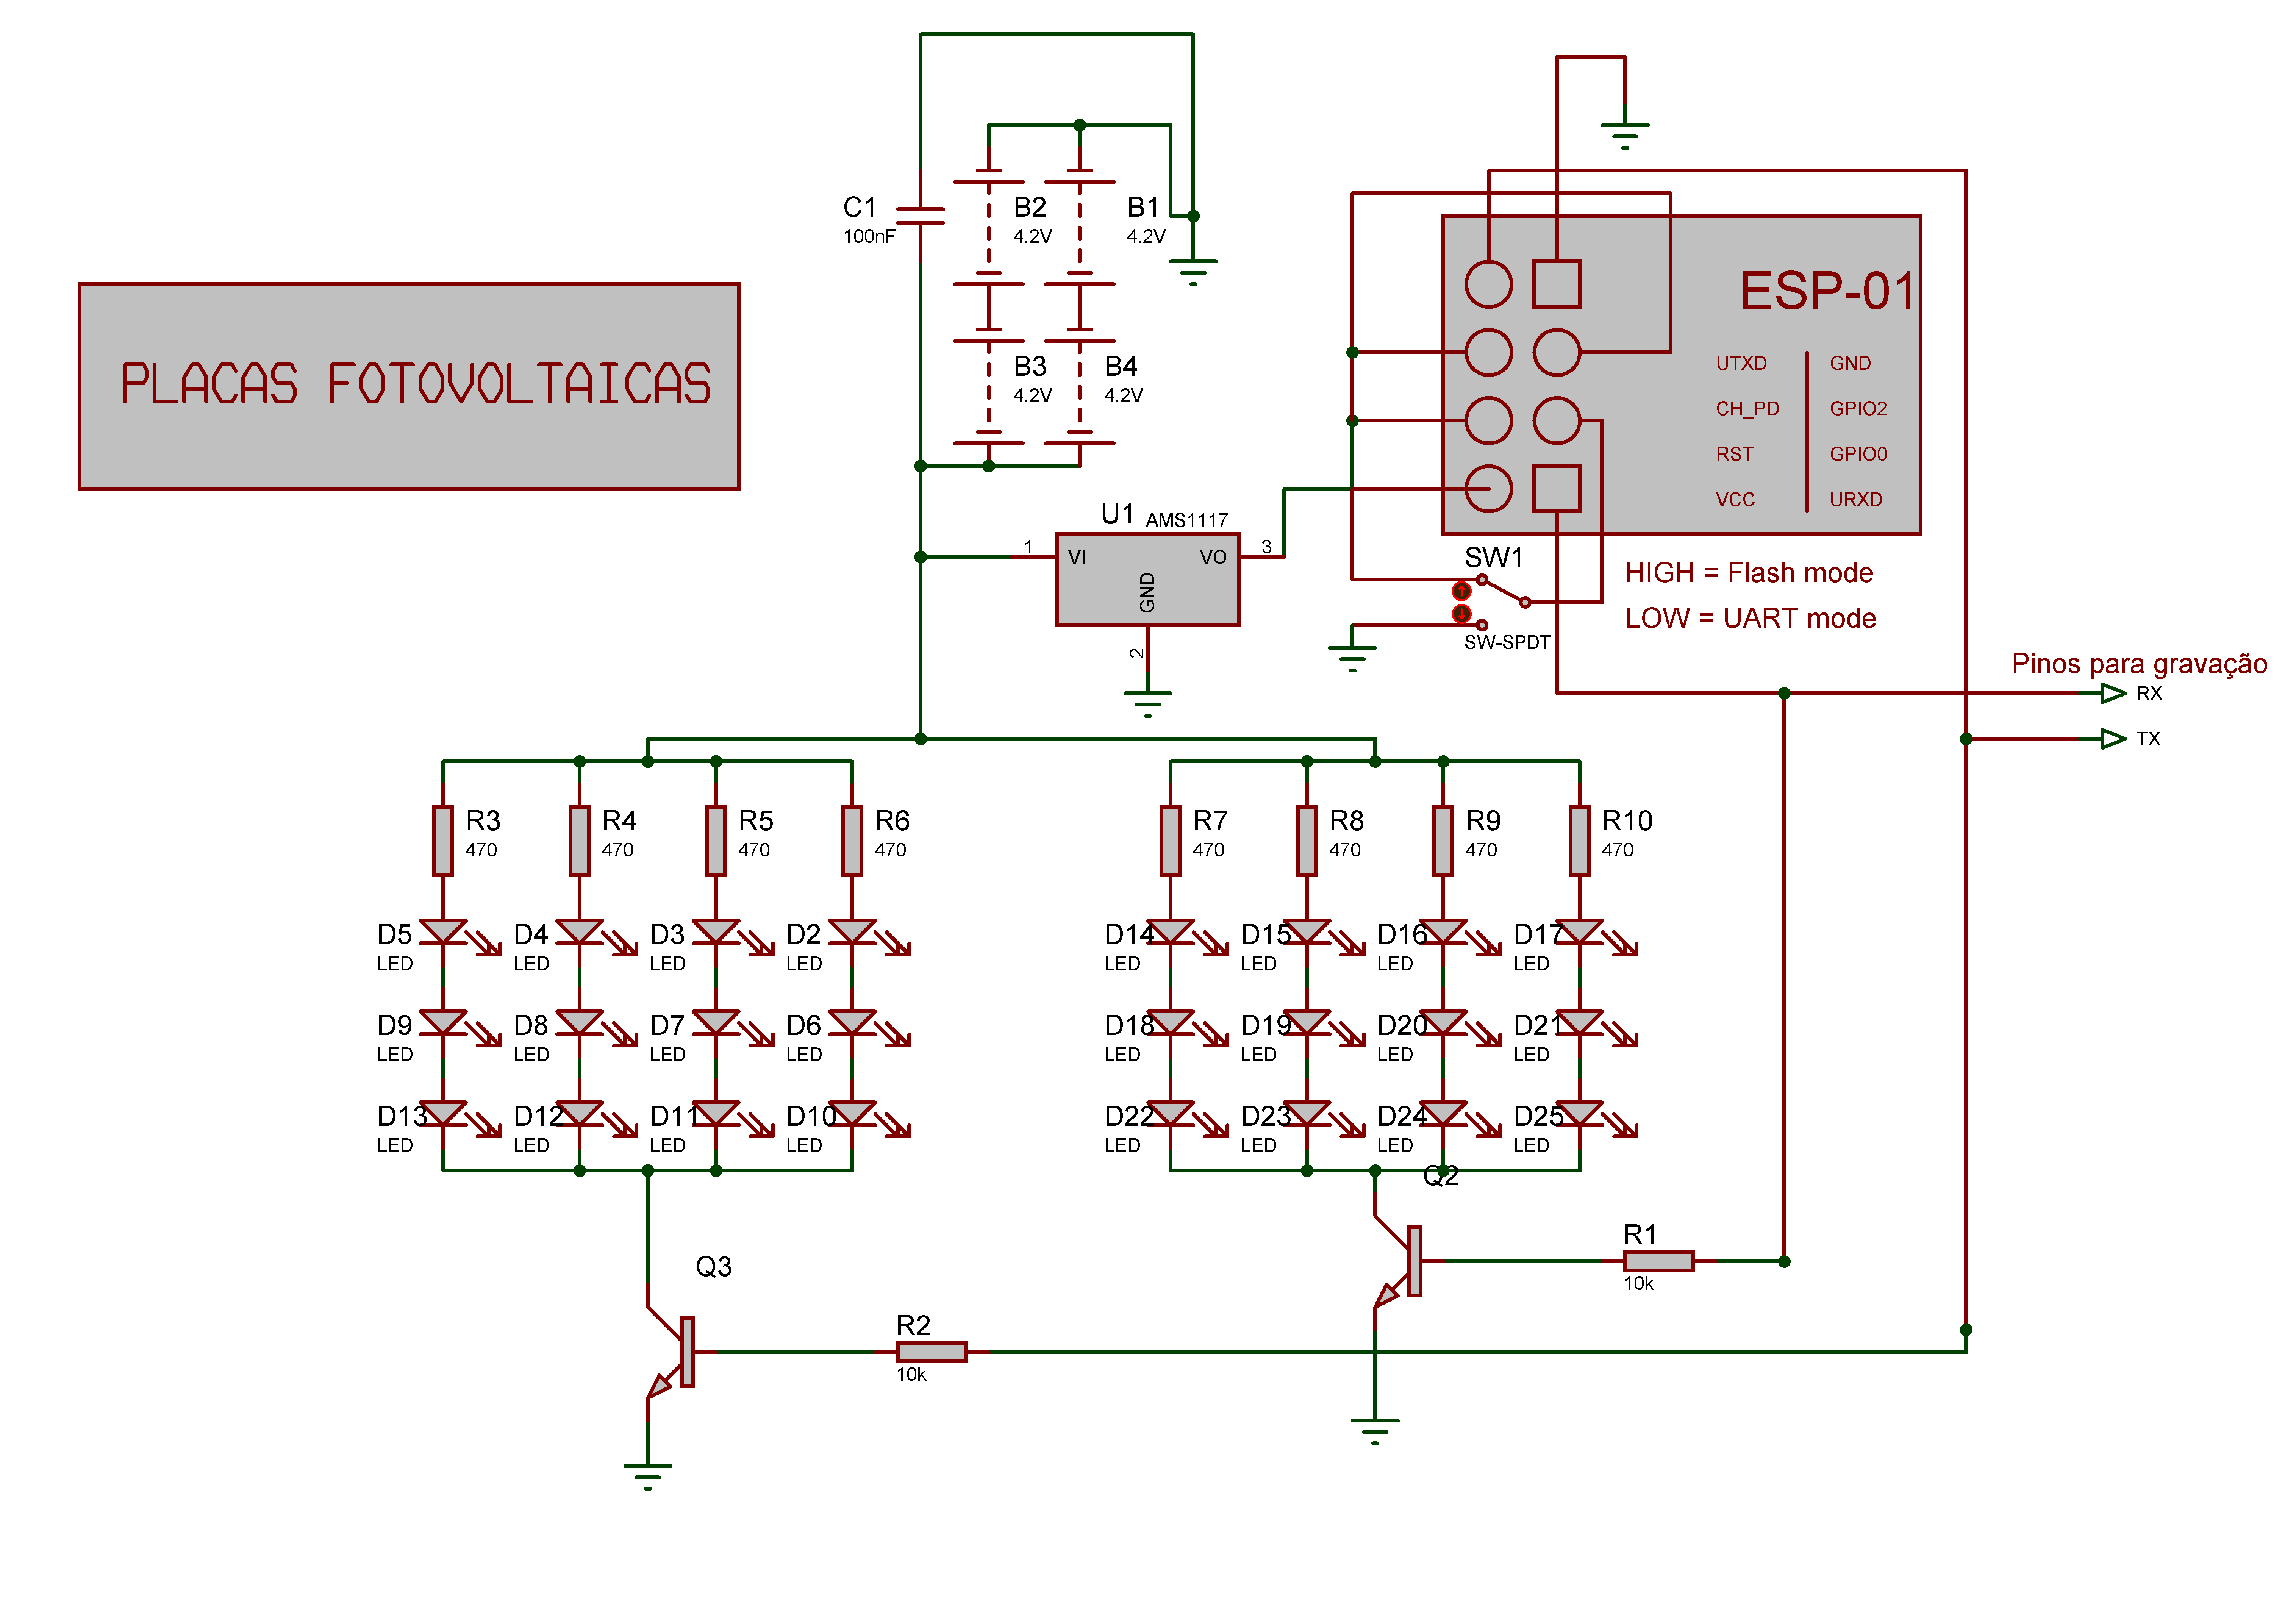
\includegraphics[width=450pt]{images/circuit.png}
  \caption{Foto do protótipo montado}
\end{figure}

\chapter{Esp8266}
É um microcontrolador de 32-bits com modem \textit{Wi-Fi} integrado desenvolvido pela \textit{Espressif Systems}
surgido, em meados de 2014, para suprir a contínua demanda por uma plataforma que fosse de \textsf{\textbf{baixo consumo}} 
energético, \textsf{\textbf{compacta}} e de \textsf{\textbf{desempenho confiável}} na industria de \textit{IoT}.

Assim como a maioria dos modelos Arduino, o ESP possui GPIOs (Pinos de entrada e saída de propósito geral)
e suporte a PWM (Modulação por largura de pulso). O upload do firmware é feito também pela UART (RX/TX), 
porém o ESP8266 conta com upload OTA (over-the-air), que é a gravação através de uma rede.  

Seguir pontos do curso
\section{Especificações}

  \begin{table}[ ]
        \begin{tabular}{|l|l|l|}
                \hline
                     & ESP-12           & ATMEGA-328p     \\ \hline
                      Arquitetura                                                      & 32-bits          & 8-bits          \\ \hline
                     Frequência                                                       & 80 $\sim$160 MHz & 16 $\sim$20 MHz \\ \hline
                    \begin{tabular}[c]{@{}l@{}}Tensão \\ \\ de operação\end{tabular} & 2.5 $\sim$3.6V   & 1.8 $\sim$5.5V  \\ \hline
                     \begin{tabular}[c]{@{}l@{}}Memória \\ \\ Flash\end{tabular}      & 1Mb $\sim$4Mb    & 32Kb            \\ \hline
                    \begin{tabular}[c]{@{}l@{}}Memória \\ \\ RAM\end{tabular}      & 15 $\sim$26Kb*    & 2Kb            \\ \hline
                   GPIOS                                                            & 18 (17/d e 1/a)  & 20 (14/d e 6/a) \\ \hline
                  Preço                                                            & \$8,79           & \$9,99          \\ \hline
        \end{tabular}
        \caption{Especificações ESP8266 vs ATMEGA-328p}
\end{table}


\subsection{JSON}

\chapter{Raspberry pi 3}

\section{Linux}

\section{Web server}
\subsection{Laravel}
\subsection{Socket.io}

% ----------------------------------------------------------
% PARTE - preparação da pesquisa
% ----------------------------------------------------------
\part{Desenvolvimento}
\chapter{Circuito}
\begin{figure}[ht!]
  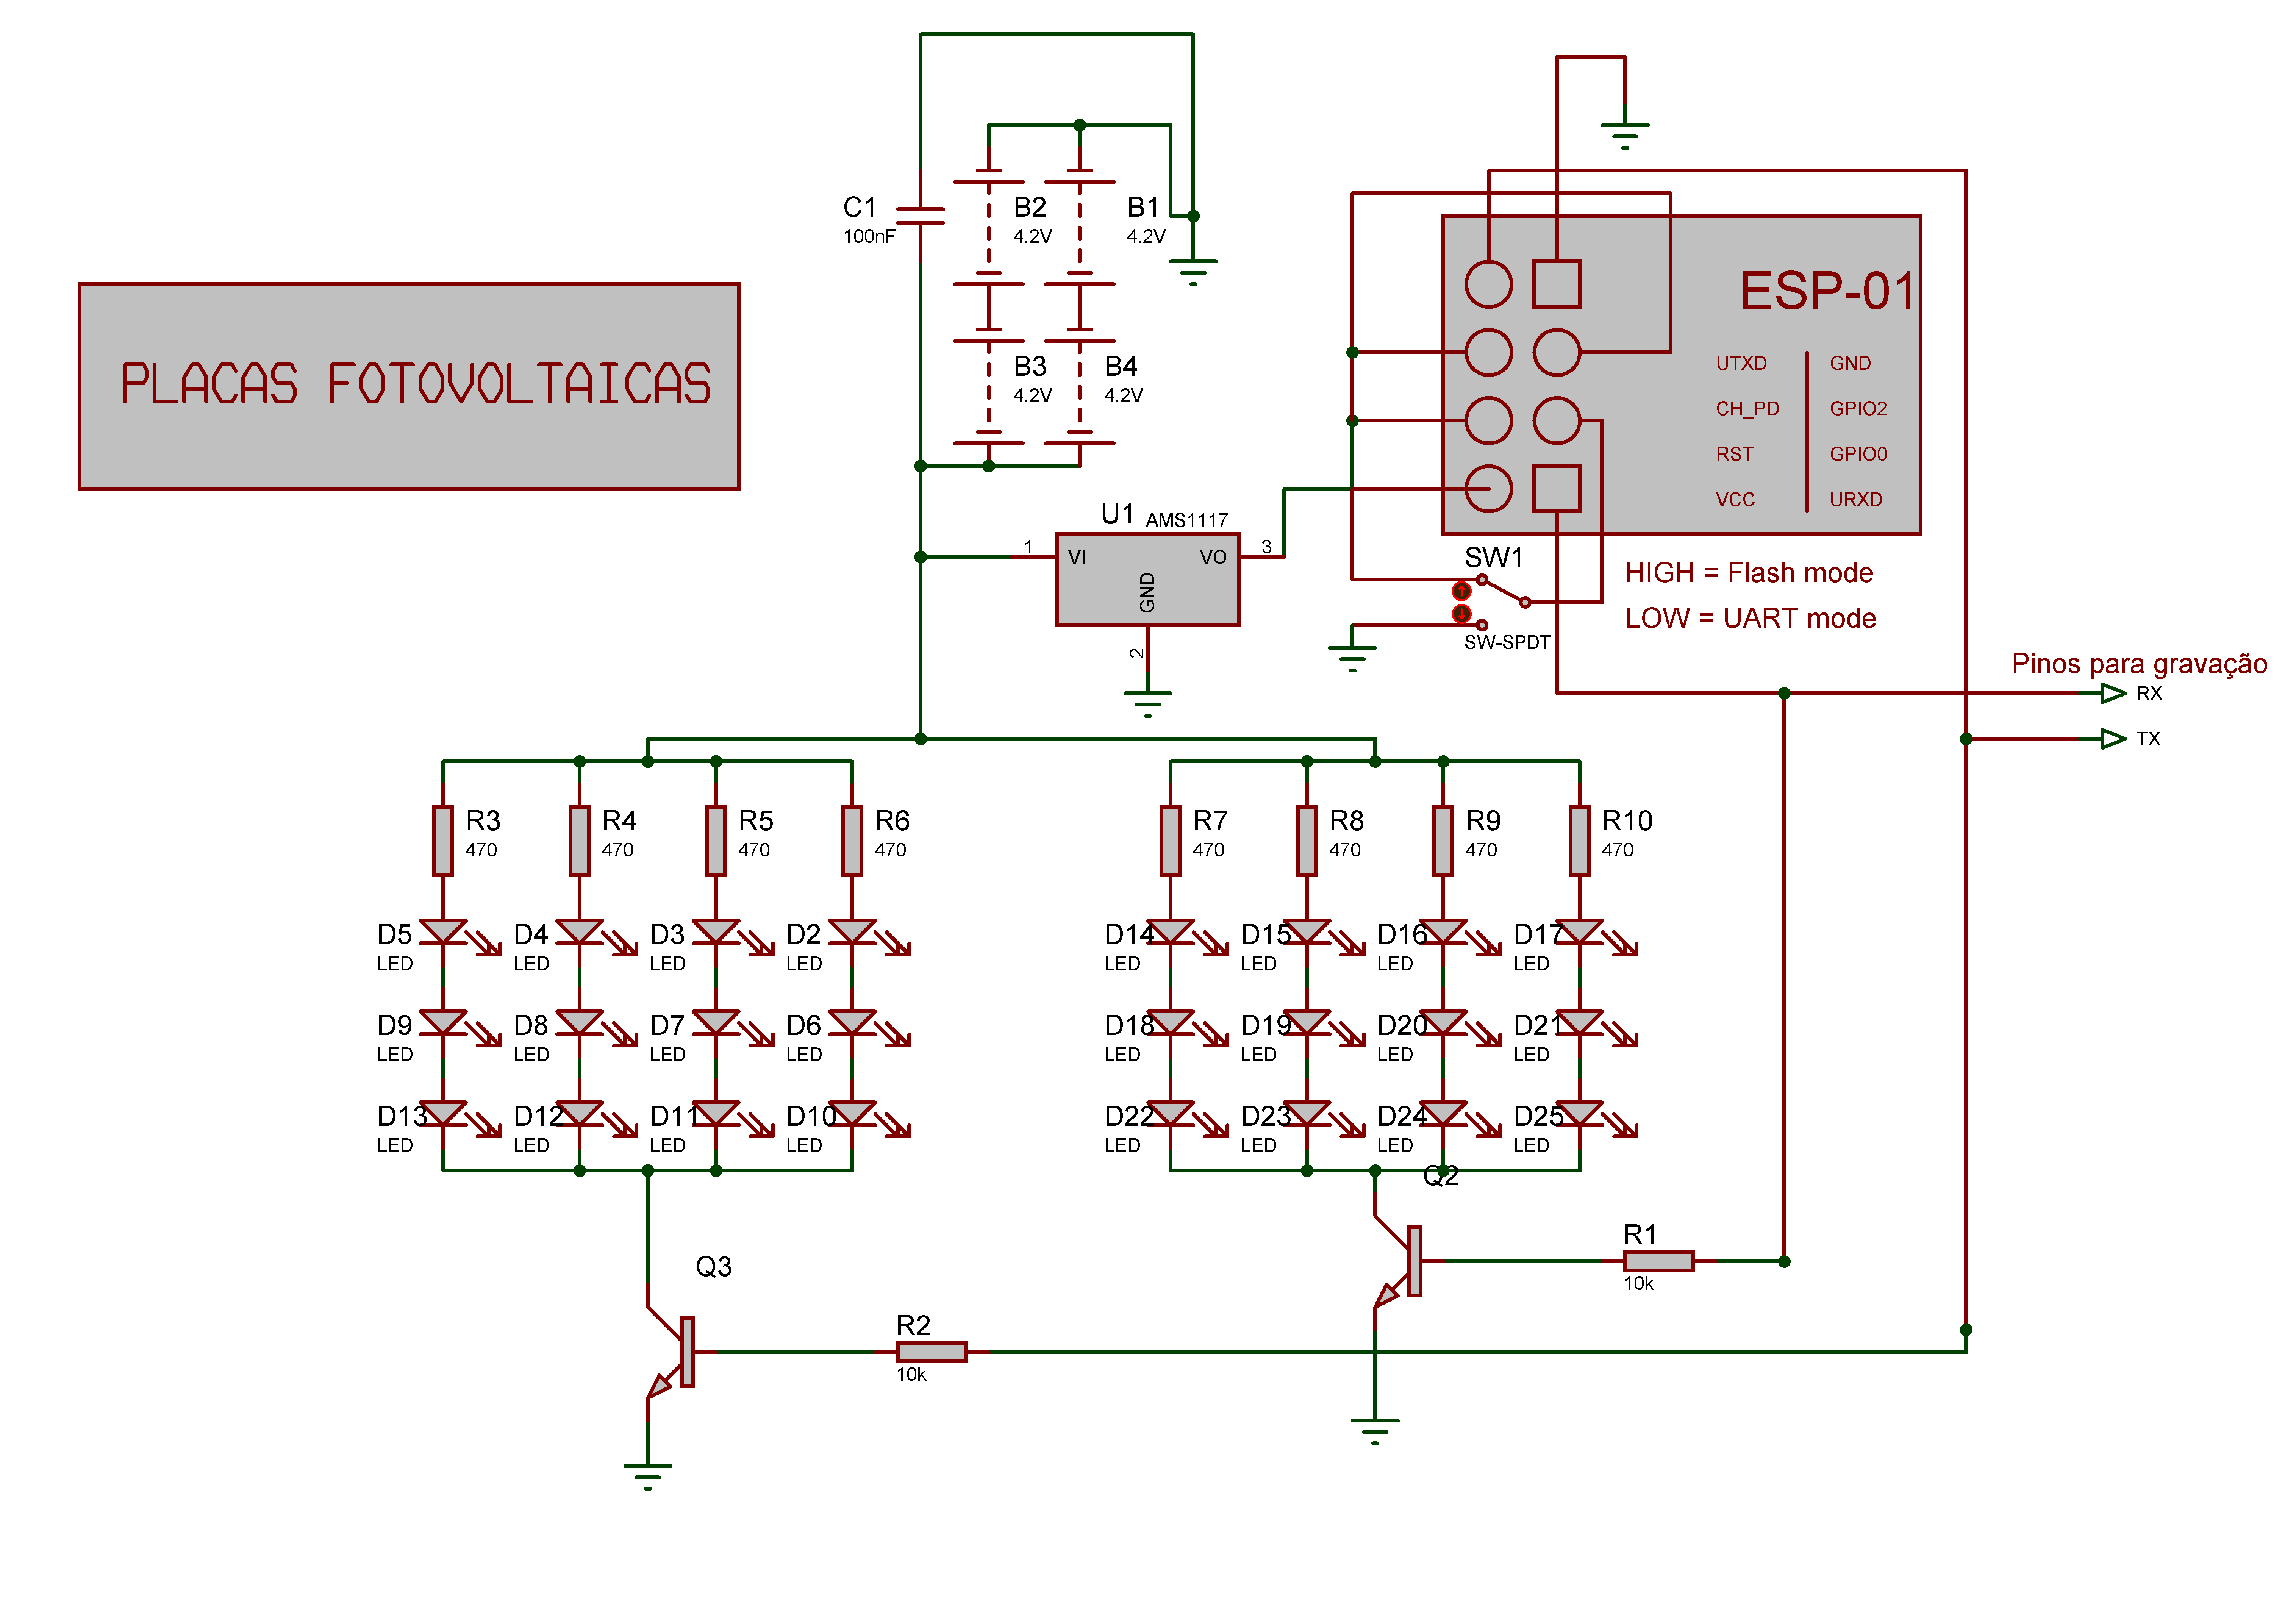
\includegraphics[width=450pt]{images/circuit.png}
  \caption{Esquemático do circuito}
\end{figure}

\section{Alimentação}
\subsection{Regulação}
\section{MCU}
\section{Placas fotovoltaicas}

% ----------------------------------------------------------
% Parte de resultados
% ----------------------------------------------------------
\part{Resultados}

% ---
% Capitulo de revisão de literatura
% ---
\chapter{Lorem ipsum dolor sit amet}

% ---
\section{Aliquam vestibulum fringilla lorem}
% ---

\lipsum[1]

\lipsum[2-3]

% ---
% Finaliza a parte no bookmark do PDF
% para que se inicie o bookmark na raiz
% e adiciona espaço de parte no Sumário
% ---
\phantompart

% ----------------------------------------------------------
% Trabalhos futuros
% ----------------------------------------------------------
\part{Trabalhos futuros}
\chapter{Circuito}

\section{Alimentação}
\subsection{Células fotovoltaicas}

\section{Raspberry pi 3}
\subsection{Web server}
Mais leve

Raspberry por um host contratado

% ---
% Conclusão
% ---
\chapter{Conclusão}
% ---

\lipsum[31-33]

% ----------------------------------------------------------
% ELEMENTOS PÓS-TEXTUAIS
% ----------------------------------------------------------
\postextual

% ----------------------------------------------------------
% Referências bibliográficas
% ----------------------------------------------------------
\bibliography{abntex2-modelo-references}

% ----------------------------------------------------------
% Glossário
% ----------------------------------------------------------
%
% Consulte o manual da classe abntex2 para orientações sobre o glossário.
%
%\glossary

% ----------------------------------------------------------
% Apêndices
% ----------------------------------------------------------

% ---
% Inicia os apêndices
% ---
\begin{apendicesenv}

% Imprime uma página indicando o início dos apêndices
\partapendices

% ----------------------------------------------------------
\chapter{Quisque libero justo}
% ----------------------------------------------------------

\lipsum[50]

% ----------------------------------------------------------
\chapter{Nullam elementum urna vel imperdiet sodales elit ipsum pharetra ligula
ac pretium ante justo a nulla curabitur tristique arcu eu metus}
% ----------------------------------------------------------
\lipsum[55-57]

\end{apendicesenv}
% ---


% ----------------------------------------------------------
% Anexos
% ----------------------------------------------------------

% ---
% Inicia os anexos
% ---
\begin{anexosenv}

% Imprime uma página indicando o início dos anexos
\partanexos

% ---
\chapter{Morbi ultrices rutrum lorem.}
% ---
\lipsum[30]

% ---
\chapter{Cras non urna sed feugiat cum sociis natoque penatibus et magnis dis
parturient montes nascetur ridiculus mus}
% ---

\lipsum[31]

% ---
\chapter{Fusce facilisis lacinia dui}
% ---

\lipsum[32]

\end{anexosenv}

%---------------------------------------------------------------------
% INDICE REMISSIVO
%---------------------------------------------------------------------

\phantompart

\printindex

%---------------------------------------------------------------------
% Formulário de Identificação (opcional)
%---------------------------------------------------------------------
\chapter*[Formulário de Identificação]{Formulário de Identificação}
\addcontentsline{toc}{chapter}{Exemplo de Formulário de Identificação}
\label{formulado-identificacao}

Exemplo de Formulário de Identificação, compatível com o Anexo A (informativo)
da ABNT NBR 10719:2015. Este formulário não é um anexo. Conforme definido na
norma, ele é o último elemento pós-textual e opcional do relatório.

\bigskip

\begin{tabular}{|p{9cm}|p{5cm}|}
\hline
\multicolumn{2}{|c|}{\textbf{\large Dados do Relatório Técnico e/ou científico}}\\
\hline
\multirow{4}{10cm}[24pt]{Título e subtítulo}& Classificação de segurança\\
                   & \\
                   \cline{2-2}
                   & No.\\
                   & \\
				
\hline
Tipo de relatório & Data\\
\hline
Título do projeto/programa/plano & No.\\
\hline
\multicolumn{2}{|l|}{Autor(es)} \\
\hline
\multicolumn{2}{|l|}{Instituição executora e endereço completo} \\
\hline
\multicolumn{2}{|l|}{Instituição patrocinadora e endereço completo} \\
\hline
\multicolumn{2}{|l|}{Resumo}\\[3cm]
\hline
\multicolumn{2}{|l|}{Palavras-chave/descritores}\\
\hline
\multicolumn{2}{|l|}{
Edição \hfill No. de páginas \hfill No. do volume \hfill Nº de classificação \phantom{XXXX}} \\
\hline
\multicolumn{2}{|l|}{
ISSN \hfill \hfill Tiragem \hfill Preço \phantom{XXXXXXXX}} \\
\hline
\multicolumn{2}{|l|}{Distribuidor} \\
\hline
\multicolumn{2}{|l|}{Observações/notas}\\[3cm]
\hline
\end{tabular}

\end{document}
